\documentclass[conference]{IEEEtran}
\IEEEoverridecommandlockouts
% The preceding line is only needed to identify funding in the first footnote. If that is unneeded, please comment it out.
\usepackage{cite}
\usepackage{amsmath,amssymb,amsfonts}
\usepackage{algorithmic}
\usepackage{graphicx}
\usepackage{textcomp}
\usepackage{xcolor}
\def\BibTeX{{\rm B\kern-.05em{\sc i\kern-.025em b}\kern-.08em
		T\kern-.1667em\lower.7ex\hbox{E}\kern-.125emX}}
\begin{document}
	
	\title{Loan Approval Prediction\\
	
	}
	\author{\IEEEauthorblockN{1\textsuperscript{st} Shravani Akolkar}
		\IEEEauthorblockA{\textit{Department of Computer Engineering} \\
			\textit{Sanjivani college of Engineering}\\
			Kopargaon, India \\
			shrauakolkar29@gmail.com}
		\and
		\IEEEauthorblockN{2\textsuperscript{nd} Yashodeep Bhamare}
		\IEEEauthorblockA{\textit{Department of Computer Engineering} \\
			\textit{Sanjivani college of Engineering}\\
			Kopargaon, India \\
			yashodeepbhamare567@gmail.com}
		\and
		\IEEEauthorblockN{3\textsuperscript{rd} Vidya Bombe}
		\IEEEauthorblockA{\textit{Department of Computer Engineering} \\
			\textit{Sanjivani college of Engineering}\\
			Kopargaon, India \\
			vidyabombe21@gmail.com}
		\and
		\IEEEauthorblockN{4\textsuperscript{th} Shubham Chaudhari}
		\IEEEauthorblockA{\textit{Department of Computer Engineering} \\
			\textit{Sanjivani college of Engineering}\\
			Kopargaon, India \\
			chaudharishubham2309@gmail.com}
	}
	
	\maketitle
	
	\begin{abstract}
	 
As technology evolves, more people are applying for loans, creating a challenge for banks to decide who should get approved. Manual assessment of each applicant is slow and risky\cite{p5}. To solve this, we use machine learning to predict if someone is a safe bet for a loan based on past records. We use techniques like logistic regression and random forest to analyze loan data and predict if an applicant is likely to be a good borrower. This study aims to help banks make better decisions by automating the process and reducing risk. By comparing the accuracy of logistic regression, random forest, decision Tree classifier, KNearestNeighbors model 
our model becomes a practical tool for improving loan approval in the banking industry.
\end{abstract}

\begin{IEEEkeywords}
Keywords:Loan Dataset, Logistic Regression, Random Forest, decision Tree classifier, KNearestNeighbors  Creditworthiness, Machine Learning, Risk Mitigation, Loan Approval, Predictive Model, Banking Sector
\end{IEEEkeywords}
	\section{Introduction}
The banking and finance industry has a lot of data, thanks to advances in technology making data collection easier and cheaper [1]. Banks are investing in ways to collect data that are both cost-effective and detailed. Even if some banks aren't fully embracing these methods, they still generate a lot of data through their everyday operations, which can be used for smart decision-making to improve efficiency and profits [2].

Loans are a big part of what banks do, and as technology improves, more people are applying for loans. This means banks have even more data to work with when making decisions about who gets approved for loans. But choosing the right people to lend to is tricky, and each bank has its own way of doing things, which adds to the challenge. Plus, finding and training people to make these decisions also costs money and comes with risks.  

The dataset we have used is from kaggle where it consists of total 614 entries with 13 attributes. The attributes in the dataset are \textit{Loan id, gender, married, dependents, education, self-employed, applicant income, co-applicant income, loan amount, loan amount term, credit history, property area, loan status}.

In the world of banking, deciding who gets approved for a loan is a crucial task\cite{p3}. To make this decision, banks often turn to advanced classification algorithms like Logistic Regression, Random Forest, Decision Tree Classifier, and KNearestNeighbors. These algorithms analyze various factors such as income, credit history, and personal details to predict whether someone is likely to repay their loan. In this project we're exploring how these algorithms can help banks make better decisions about loan approvals. By using sophisticated techniques like Logistic Regression and Random Forest, banks can assess applicants' likelihood of loan repayment more accurately. This not only streamlines the loan approval process but also reduces the risk of lending to unreliable borrowers\cite{p4}. We will investigate into the role of these algorithms in predicting loan approvals and how they contribute to making the banking sector more efficient and secure.
	\section{Literature Review}
	
	Mohammad \textit{et al.}\cite{p1} investigated different model like Logistic Regression, SVM and KNN. Among this they choose the popular and very useful algorithm 
	of machine learning for classification problems that is Logistic regression with the best accuracy. The advantage 
	of logistic regression is that it is a predictive analysis. It is 
	used for description of data and use to explain relationship 
	between a single binary variable and single or multiple 
	nominal, ordinal and ration level variables which are 
	independent in nature. 
	The model development for the prediction is taken in 
	account using the sigmoid function in logistic regression as the 
	outcome is targeted binary either 0 or 1. The dataset of 
	bank customers has been divided into training and test data 
	sets. The train dataset contains approximately 600+ rows and 
	13+ columns whereas the test dataset contains 300+ rows and 
	12+ columns, the test dataset does not contain the target 
	variable. Both the datasets are having missing values in their 
	rows, and the mean, median or mode is used to fill the missing 
	values but not removing the rows completely because the 
	datasets are already small. Using the Feature Engineering 
	techniques, the project is further proceeded and move towards 
	the exploratory data analysis, where the dependent and 
	independent variable is studied through statistics concepts such 
	normal distribution, Probability density function etc. Study of 
	the univariate, bivariate and multivariate analysis will give the 
	view of the inside dependent and independent variable. The model is focusing on to target those customers who are eligible for loans and therefore the logistic regression is enabled using the sigmoid function as it divided the probability 
	into binary output. Therefore the Prediction model can be 
	developed.\\
	
	%Design and Simulation of Loan ApprovalPrediction Model using AWS Platform
	Ramchandra \textit{et al.}\cite{p2} investigated This project aims to enhance loan approval systems by leveraging Machine Learning algorithms, particularly Decision Tree, Logistic Regression, and Random Forest. By analyzing demographic information, the project seeks to predict whether customers will repay their loans or not. Through the use of Cloud-based platforms, the model's deployment becomes more scalable, affordable, and accessible, aligning with industry trends favoring such technologies for their ease of use and flexibility. The dataset undergoes thorough testing and training, with Logistic Regression Confusion matrix analysis showing promising results, achieving an accuracy of 76. This approach represents a significant step forward in improving loan prediction systems, offering a more accurate and efficient means of assessing loan applicants' creditworthiness.\\
	
	\section{Proposed System}
	The below system diagram shows the system architecture of loan approval prediction using machine learning. The steps required to predict loan approved or rejected involves 6 steps this includes.
	
	
	\begin{document}
		
		\begin{figure}[htbp]
			
			\centering
			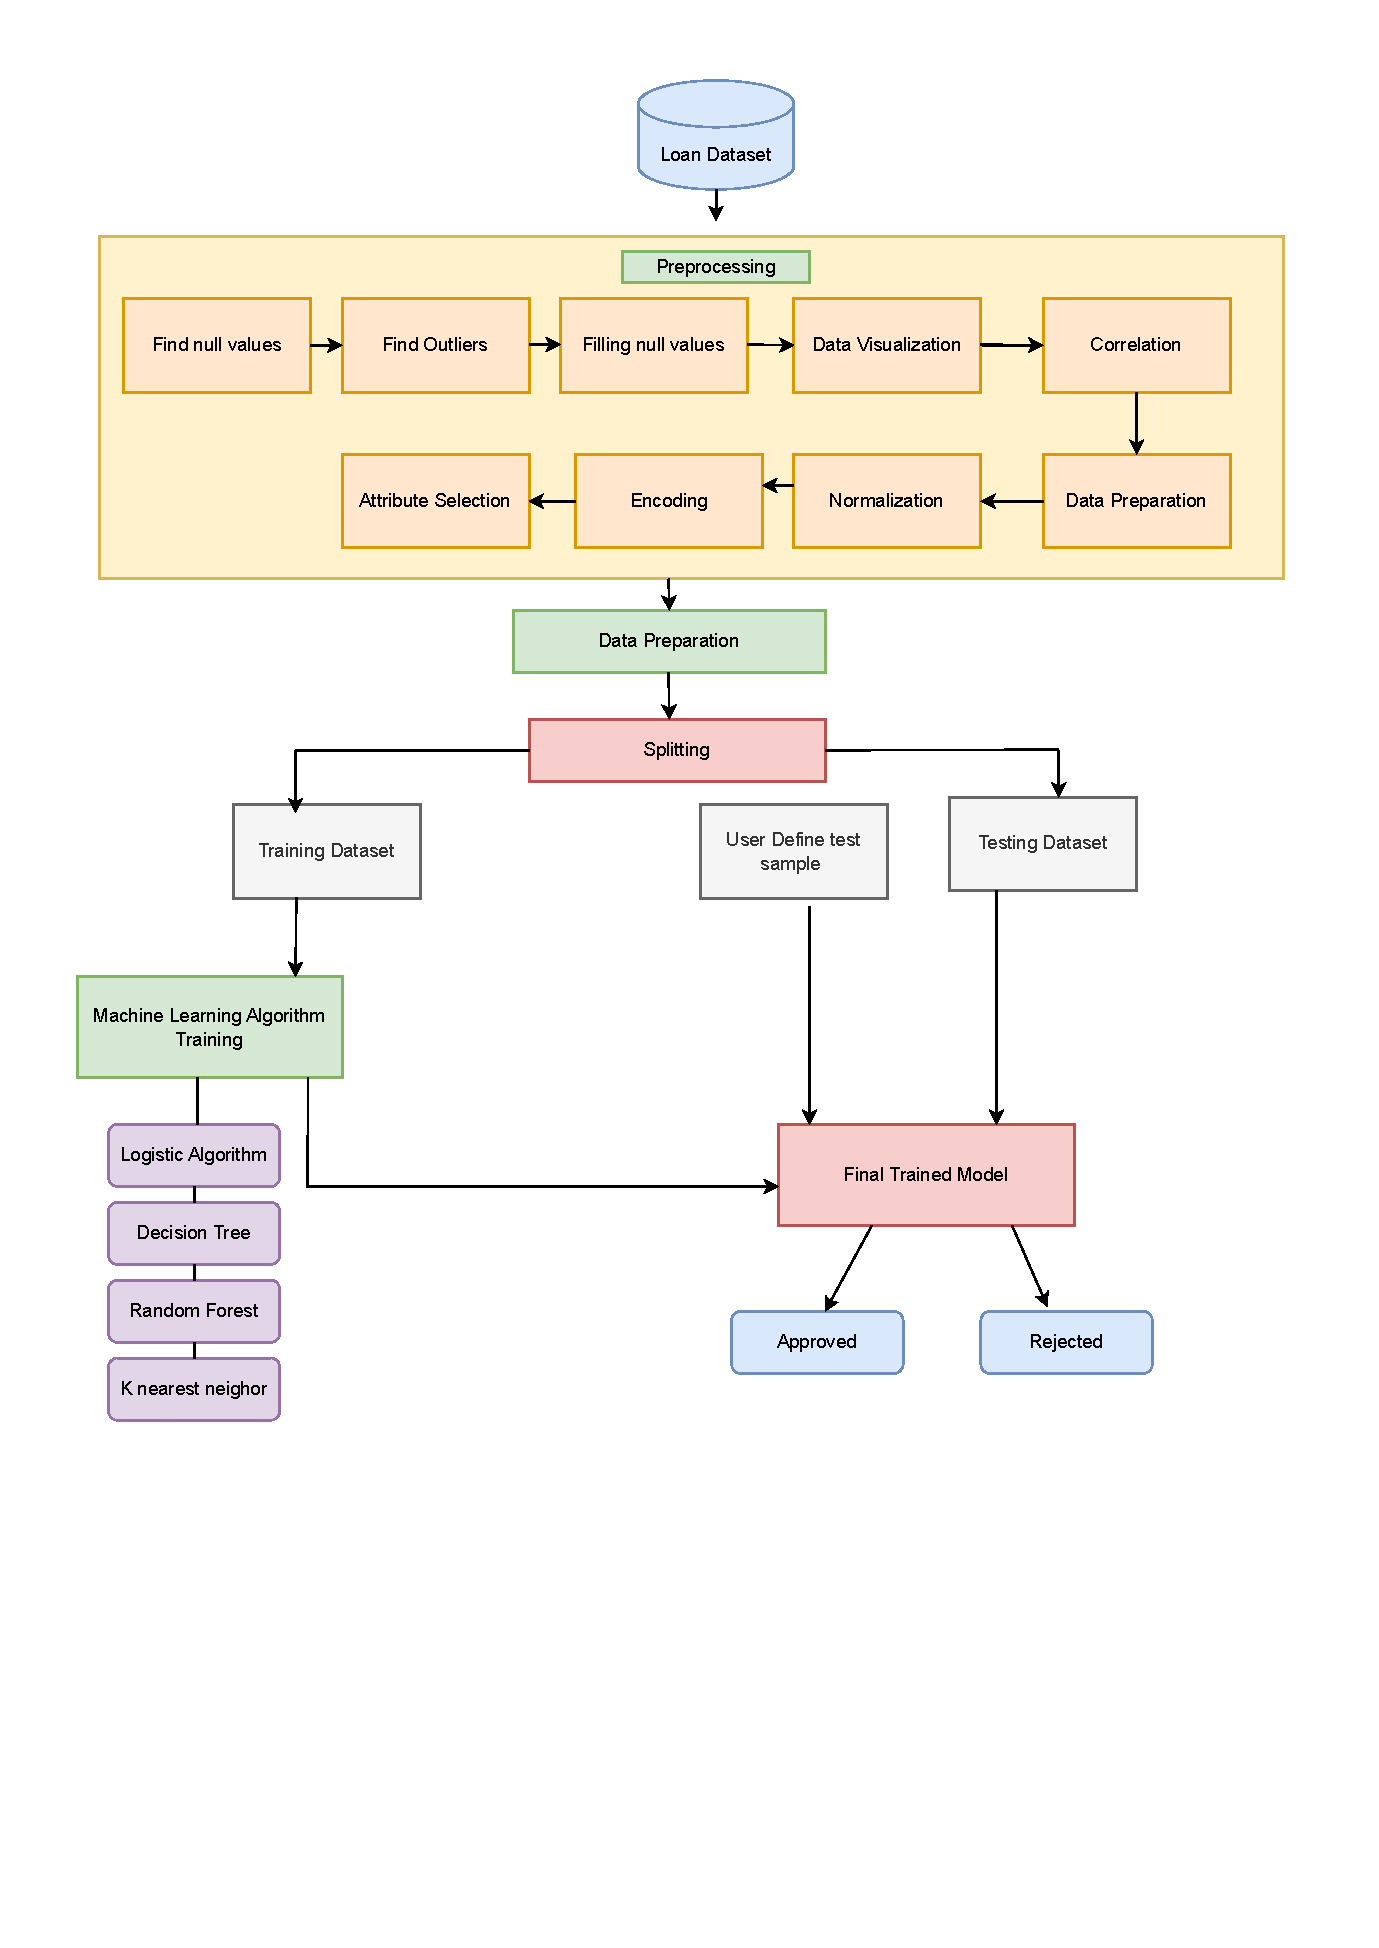
\includegraphics[width=3.3in,height=3.7in]{final architecture 02.pdf}
			\caption{System Architecture}
			\label{fig:example}
		\end{figure}
		
	
	
	\subsection{Data Collection}\label{AA}
	As in the process of data mining data collection is main step. The dataset we have considered is loan dataset which is available on  kaggle. Where the loan dataset consists of  total 614 tuples and 13 attributes. As the below table shows all 13 attributes along with it type whether numerical or object.
	\begin{table}[htbp]
		\caption{Variables in the dataset and their explanation for predicting Loan Approval}
		\begin{center}
			\renewcommand{\arraystretch}{1.5} % Adjust the value to increase or decrease the height
			\begin{tabular}{|c|c|}
				\hline
				\textbf{Variable} & \textbf{Explanation} \\
				\hline
				Loan\_ID & Unique ID \\
				\hline
				Gender & Male/Female \\
				\hline
				Self\_Employed & Self-Employed (Yes/No) \\
				\hline
				Dependents & Number of Dependents \\
				\hline
				Marital\_Status & Applicant Married (Yes/No) \\
				\hline
				Education\_Qualification & Graduate/Non graduate \\
				\hline
				Applicant\_Income & Applicant Income \\
				\hline
				Co\_Applicant\_Income & Co-Applicant Income \\
				\hline
				Loan\_Amount & Loan Amount \\
				\hline
				Loan\_Amount\_Term & Loan Term \\
				\hline
				Credit\_History & Credit History meets guidelines \\
				\hline
				Property\_Area & Urban/Semiurban/Rural \\
				\hline
				Loan\_Status & Loan Approved (Yes/No) \\
				\hline
				\multicolumn{2}{l}{$^{\mathrm{}}}
			\end{tabular}
			\label{tab1}
		\end{center}
	\end{table}
	
	
	\subsection{Data Preprocessing}
	\\
     \textbf{ \\1) Finding Null Values:}
	         During the pre-processing phase of the loan approval dataset, missing values were detected in several attributes. Specifically, key attributes such as gender, marital status, number of dependents, employment status, loan amount, loan term, and credit history had missing information for various applicants. For instance, gender information was absent for 13 applicants, while 3 applicants lacked marital status data. Additionally, 15 applicants had missing values for dependents, 32 for self-employment status, 22 for loan amount, 14 for loan term, and 50 for credit history. Handling these missing values appropriately is crucial to ensure the accuracy and reliability of subsequent analyses and modeling tasks.
	         \\
	    \\\textbf{2) Finding Outliers:}
	           
	           \begin{figure}[htbp]
	           	
	           	\centering
	           	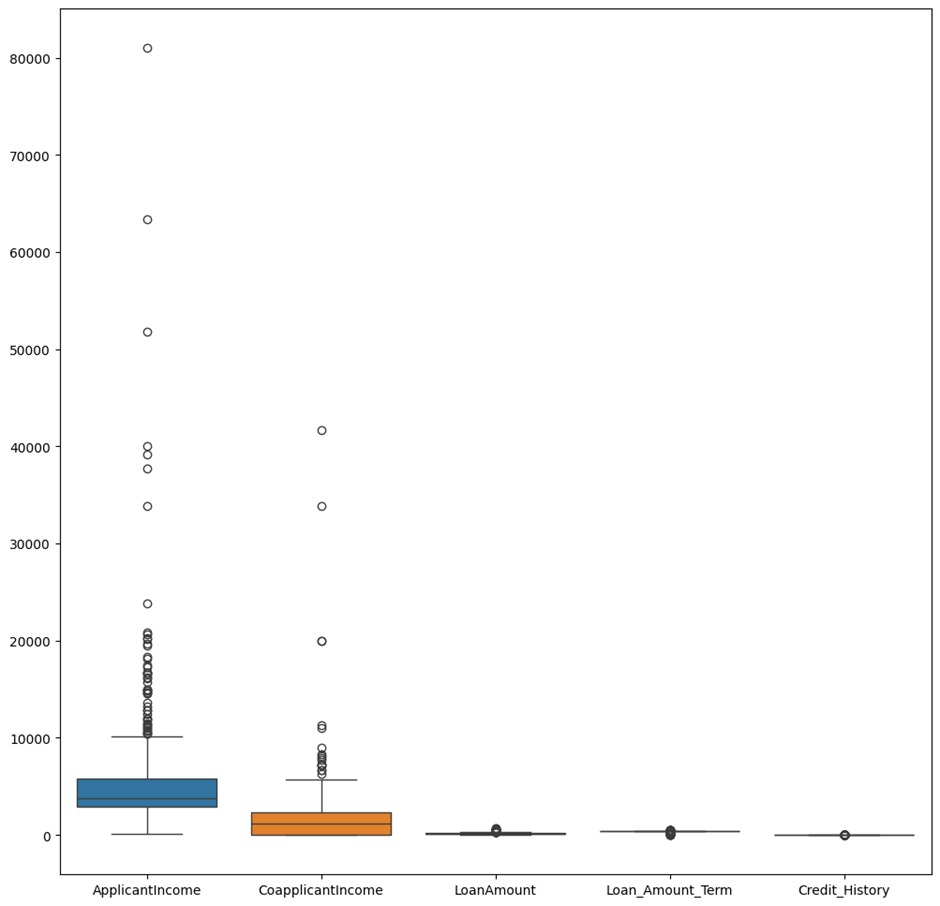
\includegraphics[width=3.3in,height=3.5in]{out.jpg}
	           	\caption{Outliers Graph}
	           	\label{fig:example}
	           \end{figure}
	           
	          In the loan approval dataset, outliers were identified in the "ApplicantIncome" attribute, which is a numerical variable. Given the presence of numerous attributes in the dataset, a decision was made to address missing values specifically in numerical data types. Since "ApplicantIncome" is a numerical attribute with outliers, strategies such as mean, median, or mode imputation can be considered to fill the null values. These methods involve replacing missing values with the mean (average), median (middle value), or mode (most frequent value) of the respective attribute. This approach ensures that the missing values are replaced with reasonable estimates, thereby preserving the integrity of the dataset for subsequent analyses and modeling tasks.
	          \\
	          \\
	          \\
	          \\
	          \\
	      \\\textbf{3) Data Visualization:}
	           The attributes in the dataset are visualize by using graphs.
	           \\a) Gender:
	           
	           \begin{figure}[htbp]
	           	
	           	\centering
	           	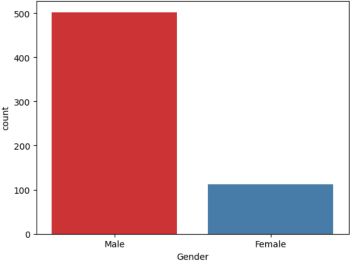
\includegraphics[width=3.3in,height=2.5in]{outlier.png}
	           	\caption{Gender Graph}
	           	\label{fig:example}
	           \end{figure}
	      It prints the count of loan applicants categorized by gender. It visualizes the count of loan applicants by gender using a countplot. From this we came to know male count is 502 and female count is 112 out of 614.
	      \\
	      \\b) Married:
	      It prints the count of loan applicants categorize by marital status. It visualizes the count of loan applicants by marital status using a count plot. From this visualization we came to know married loan appliers are 401 and unmarried are 213.
	      \begin{figure}[htbp]
	      	
	      	\centering
	      	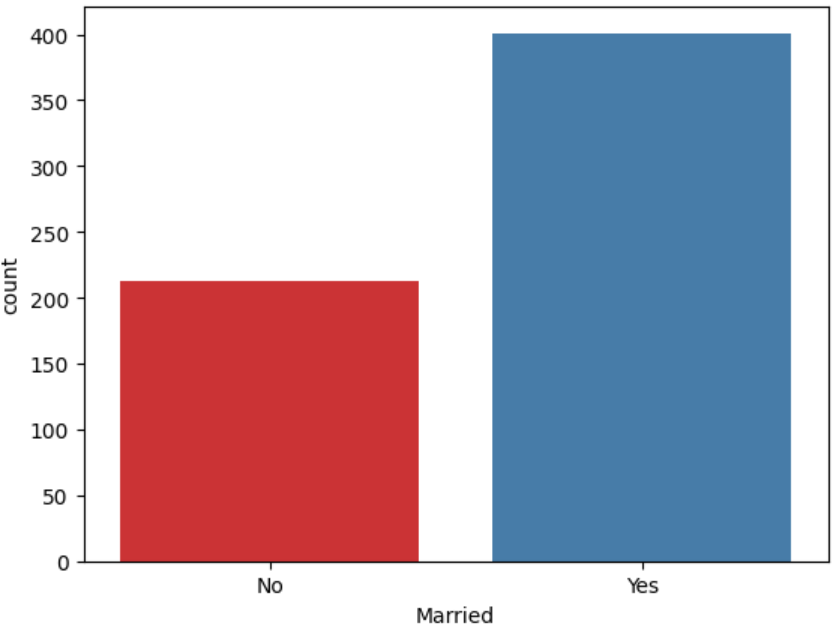
\includegraphics[width=3.3in,height=2.5in]{married.png}
	      	\caption{Married Graph}
	      	\label{fig:example}
	      \end{figure}\textbf{}
	      
	      
	      \\
	      \\c) Education:
	      It prints the count of loan applicant's categorized by their education status (graduate or not graduate).
	      It visualizes the count of loan applicants by their education status using a count plot. From this visualization we came to know their are 480 graduate and 134 non gradate.
	      \begin{figure}[htbp]
	      	
	      	\centering
	      	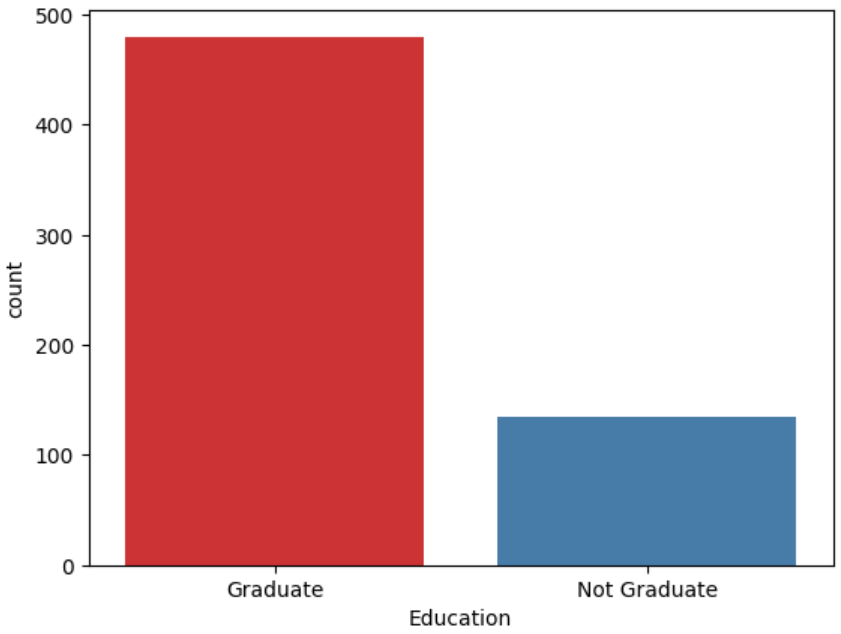
\includegraphics[width=3.3in,height=2.5in]{education.png}
	      	\caption{Education Graph}
	      	\label{fig:example}
	      \end{figure}\textbf{}
	      
	   \\\textbf{4) Finding Correlation (Heatmap):}
	   \\The correlation matrix provided represents the correlation coefficients between different pairs of attributes in the loan approval dataset. Here's a detailed explanation of the correlation matrix:
	   
	   Loan-ID: As this column only contains identifiers (IDs), it has NaN values and is not considered in the correlation analysis.
	   Gender, Married, Dependents, Education, Self-Employed, Property-Area: These categorical attributes are encoded as numerical values for correlation analysis. However, the correlation coefficients for these attributes with other numerical attributes may not provide meaningful insights due to the nature of categorical data.
	   ApplicantIncome, CoapplicantIncome, LoanAmount, Loan-Amount-Term, Credit-History, Loan-Status: These numerical attributes show the correlation with other attributes.
	   Interpretation of Correlation Coefficients:
	   
	   Correlation coefficients range from -1 to 1, where:
	   1 indicates a perfect positive linear relationship,
	   0 indicates no linear relationship, and
	   -1 indicates a perfect negative linear relationship.
	   Positive Correlation: A positive correlation coefficient indicates that as one variable increases, the other variable tends to also increase. For example:
	   ApplicantIncome and LoanAmount show a positive correlation coefficient of 0.57, suggesting that higher applicant income is associated with higher loan amounts.
	   CoapplicantIncome and LoanAmount also show a positive correlation coefficient of 0.19, indicating a similar trend.
	   Negative Correlation: A negative correlation coefficient indicates that as one variable increases, the other variable tends to decrease. For example:
	   Education and ApplicantIncome exhibit a negative correlation coefficient of -0.14, suggesting that higher levels of education are associated with lower applicant income.
	   Weak Correlation: Correlation coefficients close to 0 indicate a weak linear relationship between variables. For example:
	   Credit-History and Property-Area have correlation coefficients close to 0, indicating a weak linear relationship between these attributes.
	   \begin{figure}[htbp]
	   	
	   	\centering
	   	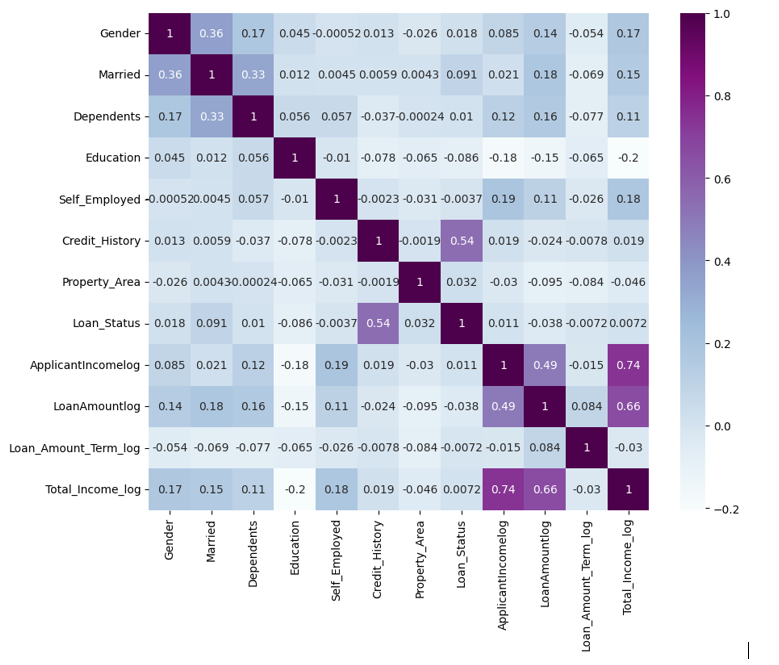
\includegraphics[width=3.7in,height=2.8in]{heatmap.png}
	   	\caption{Heatmap}
	   	\label{fig:example}
	   \end{figure}\textbf{}
	   \\
	  \\\textbf{ 5) Data Preparation:}
	  
	  The Total Income column, derived by adding the Applicant Income and Co-applicant Income, serves as a comprehensive measure of the combined financial capacity of loan applicants and their co-applicants. This aggregated figure provides a more holistic view of the household's income, crucial for evaluating loan eligibility and determining suitable loan amounts. Integrating Total Income into the dataset enhances the accuracy of loan approval predictions by capturing the collective earning potential of all applicants involved, thereby facilitating more informed decision-making in the loan approval process.
	  \\
	  \\\textbf{6)Normalization:}
	  
	  \underline{a) Applicant income}
	  Log transformation involves applying the natural logarithm function to each value in the 'ApplicantIncome' column.
	  \\
	  \underline{b) Total Income:}
	  Log transformation is applied to the 'Total Income' column by taking the natural logarithm of the sum of 'ApplicantIncome' and 'CoapplicantIncome'.
	  This transformation helps normalize the distribution of total income values, making it more symmetrical and suitable for analysis.
	  Log transformation mitigates the impact of extreme values and improves the interpretability of the total income data.
	  \\
	  \underline{c) Loan Amount Term:}
	  Log transformation is applied to the 'Loan Amount Term' column by taking the natural logarithm of the loan term values.
	  This transformation aims to normalize the distribution of loan term values, making them more suitable for modeling and analysis.
	  Log transformation helps address skewness in the loan term data and improves the performance of statistical models.
	  \\
	  \underline{d) Loan Amount:}
	  Log transformation is applied to the 'Loan Amount' column by taking the natural logarithm of the loan amount values.
	  This transformation aims to normalize the distribution of loan amount values, reducing skewness and improving model performance.
	  Log transformation helps handle variability and extreme values in loan amount data, enhancing the accuracy of predictions and analyses.
	  \\
	  \\\textbf{7)Encoding}
	  
	  Encoding techniques such as Label Encoding and One Hot Encoding are commonly used in machine learning to convert categorical data into numerical format, which is required by many machine learning algorithms. Here's an explanation of each technique:
	  
	 \textbf{a) Label Encoding:}
	  Label Encoding is a technique where each category in a categorical feature is assigned a unique numerical label.
	  It is suitable for ordinal categorical variables where the categories have a natural order or ranking.
	  In Label Encoding, the categories are encoded with integer values starting from 0 to (n-categories - 1), where n-categories are the number of unique categories in the feature.
	  For example, in a \textit{"Gender"} feature with categories "Male" and "Female", Label Encoding might assign the labels 0 and 1, respectively.
	  Label Encoding can be easily performed using libraries like scikit-learn's LabelEncoder.
	  \\
	  \textbf{b)One Hot Encoding:}
	  One Hot Encoding is a technique used to convert categorical variables into a binary matrix where each category becomes a separate binary feature (or column).
	  It is suitable for nominal categorical variables where there is no inherent order or ranking among the categories.
	  In One Hot Encoding, for each category in the original feature, a new binary feature is created. The binary feature is set to 1 if the sample belongs to that category, and 0 otherwise.
	  For example, in a "Color" feature with categories "Red", "Blue", and "Green", One Hot Encoding might create three binary features: "Color-Red", "Color-Blue", and "Color-Green".
	  One Hot Encoding prevents the model from misinterpreting categorical variables as ordinal, as each category is represented by a separate binary feature.
	  One Hot Encoding can be performed using libraries like pandas' get-dummies function or scikit-learn's OneHotEncoder.
	
	\\
	\\ \textbf{8) Attribute Selection: }
	
	\\
	Before feature selection:
	
	Initially, there were 11 attributes/features: \textit{'Gender', 'Married', 'Dependents', 'Education', 'Self-Employed', 'Credit-History', 'Property-Area', 'ApplicantIncomelog', 'LoanAmountlog', 'Loan-Amount-Term-log', 'Total-Income-log'.}
	After feature selection:
	
	The SelectKBest method using chi-squared test was applied to select the top 7 features based on their importance or contribution to the target variable 'y' (presumably the loan approval status).
	Out of the 11 original features, the SelectKBest method retained the 7 most significant features.
	Therefore, after feature selection, only 7 attributes remain in the dataset, which are considered the most informative or predictive for the loan approval prediction task.
	The names of the selected features are printed as 'Selected Features:', indicating the attributes that were chosen for further analysis or modeling based on their importance determined by the chi-squared test.
	\\
	\\\textbf{9) Model Splitting and Model Training}
	\\
	In the model splitting and training phase, four different machine learning algorithms were utilized: Logistic Regression, Random Forest, Decision Tree, and K Nearest Neighbors (KNN). Here are the accuracy's achieved by each algorithm:

	
	
	

	

	\section*{Methodology}
	\subsection{Logistic Regression}
	A statistical technique called logistic regression is applied to binary classification problems in which estimating the likelihood of a particular event or result occurring is the objective. It is extensively utilized in statistics and machine learning for a variety of purposes, such as determining whether or not an email is spam, if a patient has a specific illness, if a buyer would purchase a product,etc.
	\\How Logistic Regression works:
	Using the logistic function, logistic regression models the relationship between input feature probability and a binary outcome. It calculates the likelihood that a specific input falls into one of two categories. It modifies its parameters throughout training in order to reduce the discrepancy between expected and actual results. Once trained, it can categorized incoming data points according to a predetermined threshold and estimate the likelihood of each event.
	\\Steps of Logistic Regression Algorithm:
	\\1.Data Collection: Compile a dataset with the matching binary target variable and input feature pairs. 
	\\2.Data Pre-processing: Divide the data into training and testing sets, encode categorical variables, handle missing values, and scale or normalize features as needed.
	\\3.Model Initialization: Set zeros or random values as the model's initial values.
	\\4.Model Training: To minimize a cost function on the training data, iteratively update the model parameters using an optimization procedure.
	\\5.Prediction: Utilise the factors you have learned to forecast the likelihood of a result for fresh data points after training. 
	\\6.Model Evaluation: Assess the model's performance on the test set using a variety of measures, including ROC-AUC, accuracy, precision, recall, and F1-score.
	\\7.Model tuning: To enhance the model's performance, fine-tune its hyperparameters.
	\\8.Deployment: Use the model to make predictions on fresh, unobserved data if you're pleased with its performance.
	
	\subsection{Decision Tree Classifier}
	A supervised learning approach that can be applied to regression and classification problems is the decision tree classifier. It creates a tree-like structure in the context of classification, with each leaf node representing the class label or goal value and each internal node representing a choice based on the value of a feature attribute.
	
	\\Steps of Decision Tree Classifier:
	\\1.Data Preparation: Compile a dataset with associated target labels and features.
	\\2.Feature Selection: Pick the characteristic that divides the data into the most different classes. To quantify the purity of the resulting subsets, a metric such as entropy or Gini impurity is usually used.
	\\3.Splitting: Using the chosen feature as a guide, divide the dataset into smaller groups.
	\\4.Recursive Partitioning: Create decision tree branches by iteratively partitioning each subgroup until a halting requirement is satisfied.
	\\5.Leaf Node Assignment: Based on the majority class of the samples in each leaf node, assign a class label to each node when a stopping requirement is met.
	\\6.Pruning (optional): Once the entire tree has been constructed, remove any branches that don't significantly increase classification accuracy.
	\\7.Model Evaluation: On a different validation or test dataset, assess the decision tree classifier's performance using measures such as accuracy, precision, recall, F1-score, and confusion matrix.
	\\8.Model Interpretation: To understand the decision-making process of the model, visualize the decision tree.
	
	\subsection{Random Forest Classifier}
	For classification problems, an ensemble learning technique called a Random Forest classifier is employed. In order for it to function, it builds several decision trees during training and outputs the class that represents the mean prediction (regression) or mode of the classes (classification) of the individual trees.
	
	\\Steps of Random Forest Classifier:
	\\1.Data Preparation: Assemble your dataset, making sure each feature has an associated target label.
	\\2.Bootstrapping: Choose training data subsets at random using replacement.
	\\3.Feature Randomization: Choose a subset of features at random for consideration for splitting at each decision tree node. 
	\\4.Tree Construction: Using the chosen subset of features, construct a decision tree for every bootstrap sample. 
	\\5.Ensemble Learning: Build an ensemble of decision trees by repeatedly carrying out steps 2-4, resulting in a tree forest.
	\\6.Voting: Every tree in the forest independently guesses the class label for a given input during the prediction process.
	\\7.Model Evaluation: On a different validation or test dataset, assess the Random Forest classifier's performance using measures like as accuracy, precision, recall, F1-score, and confusion matrix.
	\\8.Parameter tuning: To maximize model performance, fine-tune hyperparameters such as the number of trees in the forest, the maximum tree depth, the amount of features to take into account at each split, and the minimum number of samples per leaf.
	
	\subsection{K Nearest Neighbor Model}
	For problems involving regression and classification, supervised machine learning is employed through the K Nearest Neighbors (KNN) model. Being a non-parametric and lazy learning algorithm, it doesn't explicitly learn a model during training and doesn't make any assumptions about the distribution of the underlying data. Rather, it uses all of the training data points that are stored in memory to predict the values of new data points.
	\\How K Nearest Neighbor model works:
	
	\\Steps of K Nearest Neighbor Model:
	\\1.Select the Value of K: Choose how many neighbors (K) to take into account while generating forecasts.
	\\2.Calculate Distances: Determine the separation between each new point in the training dataset and every other point. 
	\\3.Find K Nearest Neighbors: Using the calculated distances, determine which K data points in the training dataset are closest to the new data point.
	\\4.Majority Voting (Classification): Ascertain the K nearest neighbors' class labels for classification jobs. 
	\\5.Mean Calculation (Regression): Get the K nearest neighbours' target values for regression jobs. 
	\\6.Evaluation of the Model: Analyse the KNN model's performance on a different validation or test dataset using metrics like accuracy, precision, recall, F1-score, or mean squared error.
	\\7.Hyperparameter tuning: To maximize the performance of the model, experiment with various values of K and perhaps alternative distance measurements.
	
	
	\section*{Result analysis}
	
\documentclass{}
\usepackage{}
\usepackage{}


	
	\begin{table}[h]
\centering
\caption{Classification Report for Logistic Regression}
\begin{tabular}{lcccc}
\hline
 & Precision & Recall & F1-score & Support \\ \hline
0 & 0.85 & 0.54 & 0.66 & 114 \\[1ex]
1 & 0.62 & 0.89 & 0.73 & 97 \\ \hline
Accuracy & & & 0.70 & 211 \\[1ex]
Macro Avg & 0.73 & 0.71 & 0.69 & 211 \\[1ex]
Weighted Avg & 0.74 & 0.70 & 0.69 & 211 \\ \hline
\end{tabular}
\end{table}

\textbf{Analysis:} The logistic regression model shows moderate performance with an accuracy of 0.70. It performs relatively better in predicting class 1 (recall of 0.89) compared to class 0 (recall of 0.54).


	
	\begin{table}[h]
\centering
\caption{Classification Report for Decision Tree}
\begin{tabular}{lcccc}
\hline
 & Precision & Recall & F1-score & Support \\ \hline
0 & 0.78 & 0.86 & 0.82 & 114 \\[1ex]
1 & 0.81 & 0.71 & 0.76 & 97 \\ \hline
Accuracy & & & 0.79 & 211 \\[1ex]
Macro Avg & 0.79 & 0.79 & 0.79 & 211 \\[1ex]
Weighted Avg & 0.79 & 0.79 & 0.79 & 211 \\ \hline
\end{tabular}
\end{table}

\textbf{Analysis:} The decision tree classifier demonstrates good performance with an accuracy of 0.79. It has balanced precision and recall values for both classes, indicating a robust classification.


	
	
	\begin{table}[h]
\centering
\caption{Classification Report for Random Forest}
\begin{tabular}{lcccc}
\hline
 & Precision & Recall & F1-score & Support \\ \hline
0 & 0.92 & 0.86 & 0.89 & 114 \\[1ex]
1 & 0.85 & 0.91 & 0.88 & 97 \\ \hline
Accuracy & & & 0.88 & 211 \\[1ex]
Macro Avg & 0.88 & 0.88 & 0.88 & 211 \\[1ex]
Weighted Avg & 0.88 & 0.88 & 0.88 & 211 \\ \hline
\end{tabular}
\end{table}

\textbf{Analysis:} The random forest classifier stands out with its impressive performance, boasting an accuracy of 0.88. This high accuracy is a testament to its robustness in accurately classifying instances. Furthermore, the classifier demonstrates strong precision and recall values for both classes, indicating its effectiveness in distinguishing between positive and negative instances. The balanced precision and recall values underscore the classifier's capability to make accurate predictions while minimizing false positives and false negatives, thus ensuring reliable classification outcomes. Overall, the random forest classifier proves to be a powerful and versatile tool for classification tasks, particularly suited for complex datasets with multiple features and classes.



\begin{table}[h]
\centering
\caption{Classification Report for K-Nearest Neighbors}
\begin{tabular}{lcccc}
\hline
 & Precision & Recall & F1-score & Support \\ \hline
0 & 0.77 & 0.72 & 0.74 & 114 \\[1ex]
1 & 0.69 & 0.74 & 0.72 & 97 \\ \hline
Accuracy & & & 0.73 & 211 \\[1ex]
Macro Avg & 0.73 & 0.73 & 0.73 & 211 \\[1ex]
Weighted Avg & 0.73 & 0.73 & 0.73 & 211 \\ \hline
\end{tabular}
\end{table}

\textbf{Analysis:} The K-nearest neighbors (KNN) classifier, with an accuracy of 0.73, demonstrates a moderate level of performance.



\\
	\section*{Conclusion}
	\\
In conclusion, the random forest classifier performs the best among the presented algorithms, with the highest accuracy of 0.88 and strong precision and recall values for both classes. However, the decision tree classifier also performs well, closely following the random forest in terms of accuracy and balanced classification. The logistic regression model shows moderate performance, while the K-nearest neighbors classifier demonstrates comparatively lower accuracy and balanced classification.






	
        \
	\bibliographystyle{plain}
	\bibliography{mybib}
	
\end{document}